% ============================================================================================================
\chapter{Réoptimisation exploratoire}\label{ch:optimisation}
% ============================================================================================================

\begin{hypothese}[Statut de ce chapitre]
La réoptimisation reprend la méthode de la phase 3 sans la modifier : métamodèle linéaire construit sur les 68
expériences (relancées avec la v0.8), front de Pareto sur 40 000 portefeuilles, stratégies définies par un objectif et
des contraintes explicites (pas de score unique pondéré), robustesse aux préférences sur 300 jeux de poids. Les
compositions v0.8 ne sont \emph{pas} vérifiées par le modèle complet (la vérification de la phase 3 a montré des écarts
d'additivité de quelques dixièmes de point de PIB et de quelques points de dette). Elles servent à répondre à deux
questions : les solutions de la v0.7 restent-elles pertinentes ? les gagnants et les perdants sont-ils bien représentés ?
Elles ne constituent pas des recommandations.
\end{hypothese}

Deux variantes sont calculées : avec les critères distributifs de la v0.7 (microsimulation statique, « v0.8 stat. ») et
avec les critères distributifs après propagation macroéconomique (M16 : niveau de vie des trois premiers déciles,
pauvreté, Gini et médiane en revenu réel, par horizon ; « v0.8 dyn. »). Dans la seconde, les moyens des services
publics (Md€ de santé, d'éducation, de fonctionnement, d'emplois publics et de point d'indice) deviennent un critère à
part entière, comme le demande le cahier des charges ; c'est un indicateur de moyens, faute de mesure de la qualité des
services.

\section{Les solutions de la v0.7 sont-elles encore pertinentes ?}

\begin{table}[htbp]\centering\scriptsize
\caption{Composition des stratégies v0.7 et v0.8 réoptimisées (écart à la législation actuelle). 07 : v0.7 ;
08s : v0.8, distribution statique ; 08d : v0.8, distribution après propagation.}\label{tab:optim_compo}
\tabfit{../tables/optim_composition.tex}
\end{table}

\begin{table}[htbp]\centering\scriptsize
\caption{La composition optimale v0.7 évaluée avec le métamodèle v0.8 : valeur de l'objectif de la stratégie
(objectif à l'horizon 2037, 2042 pour S3), dette en 2047, contraintes violées.}\label{tab:optim_pertinence}
\tabfit{../tables/optim_pertinence.tex}
\end{table}

\paragraph{Réponse : en partie seulement.} Évaluées avec le métamodèle v0.8, les compositions optimales de la v0.7
pour S1, S2 et S3 violent leur contrainte de dette : $+9$ points en 2047 pour S1, $+6$ points en 2037 pour S2 et $+23$
points en 2042 pour S3. Elles reposaient sur les gains budgétaires que la fermeture de la v0.7 attribuait aux mesures
d'offre et d'activité. Les compositions de S4 et S5 restent admissibles avec la distribution statique ; avec la
distribution après propagation, elles violent la contrainte de perte maximale par décile (le premier décile perd
4,1 \% dans S4 et 2,3 \% dans S5), parce que la baisse de 25 \% des allocations chômage qu'elles contiennent fait
désormais apparaître ses perdants.

\paragraph{Ce qui change dans les compositions réoptimisées.} Avec la distribution statique, la v0.8 garde la
structure des solutions v0.7 (quatre à sept leviers communs sur huit) mais réduit leur ambition budgétaire. Avec la
distribution après propagation, deux changements nets apparaissent : la baisse des allocations chômage disparaît des
stratégies S3, S4 et S5 (elle n'est plus retenue que dans 1 \% des tirages de préférences, contre 33 \% en v0.7), et S1
abaisse l'âge légal à 62 ans (retenu dans 54 \% des tirages), ce qui augmente le niveau de vie des trois premiers
déciles mais coûte 2,7 \% de PIB en 2047. Le front de Pareto est plus large : 70 \% des portefeuilles aléatoires
étaient dominés en v0.7, 30 \% seulement avec la distribution dynamique, parce que les critères distributifs entrent
davantage en conflit avec les critères d'activité et de finances publiques.


\section{Front de Pareto et robustesse aux préférences}

\begin{figure}[htbp]\centering
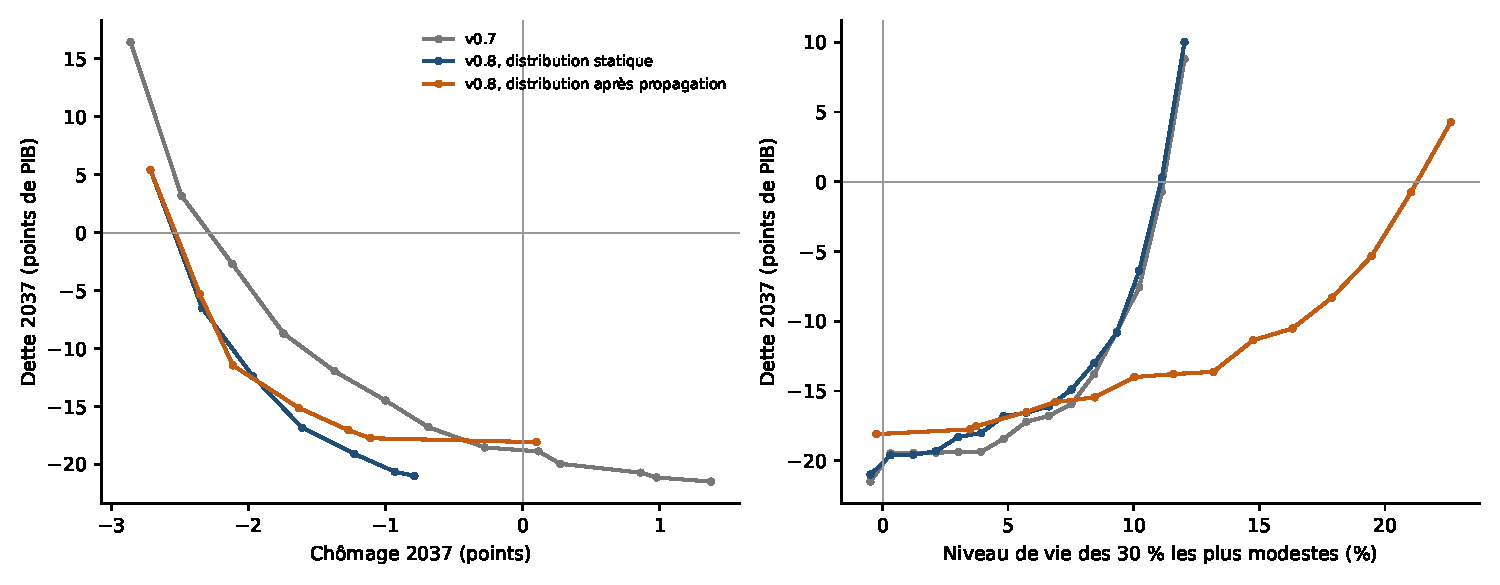
\includegraphics[width=\linewidth]{pareto_v08.pdf}
\caption{Fronts de Pareto en 2037 (périmètre principal, leviers de niveaux A et B) : v0.7, v0.8 avec distribution
statique et v0.8 avec distribution après propagation.}\label{fig:pareto_v08}
\end{figure}

\begin{table}[htbp]\centering\scriptsize
\caption{Fréquence d'emploi des leviers dans l'optimum quand les poids des critères sont tirés au hasard (300 tirages,
\%). Un levier fréquent est robuste aux préférences ; un levier rare dépend d'un choix de priorités.}\label{tab:optim_pref}
\tabfit{../tables/optim_preferences.tex}
\end{table}

\paragraph{Solutions robustes et solutions de préférence.} Sont robustes (fréquents quel que soit le jeu de poids, et
retenus dans les trois optimisations) : la hausse de la prime d'activité et du RSA, la hausse des droits de succession,
la baisse de la CSG sur les revenus d'activité. Ces leviers améliorent plusieurs critères à la fois pour un coût
budgétaire modéré ou compensé ; ils n'ont que peu de perdants (les ménages aisés pour les successions). À l'inverse, le
relèvement de l'âge légal, l'investissement public et la hausse de l'IS dépendent
des priorités : ils améliorent un critère (dette, PIB) au prix d'un autre (revenu des plus modestes, chômage à court
terme). L'âge légal est moins souvent retenu qu'en v0.7 (27 à 40 \% des tirages, contre 64 \%) parce que ses gains
budgétaires sont réduits par la fermeture estimée et que la distribution dynamique fait désormais apparaître ses
perdants. Le point d'indice est très fréquent dans la variante dynamique (77 \%), mais c'est un effet de la définition
du critère « services publics » (qui le compte comme un moyen) : il ne faut pas l'interpréter comme un résultat
économique. La baisse des allocations chômage, retenue dans un tiers des tirages en v0.7, ne l'est presque plus
quand ses perdants sont visibles (1 \%).

\begin{limites}[Ce que la réoptimisation ne dit pas]
Le métamodèle additionne les effets des leviers ; il ignore leurs interactions et les non-linéarités. Les critères de
moyens des services publics ne mesurent pas leur qualité. Les leviers de niveau C (relocalisation, durée du travail, R\&D,
formation, droits de douane) sont exclus du périmètre principal. Les bornes des leviers et les contraintes des
stratégies sont celles de la phase 3 ; d'autres bornes donneraient d'autres compositions.
\end{limites}
